\documentclass[lettersize,journal]{IEEEtran}
\usepackage{amsmath,amsfonts}
\usepackage{algorithmic}
\usepackage{algorithm}
\usepackage{array}
\usepackage[caption=false,font=normalsize,labelfont=sf,textfont=sf]{subfig}
\usepackage{textcomp}
\usepackage{url}
\usepackage{verbatim}
\usepackage{graphicx}
\usepackage{cite}
\usepackage{tikz}
\usepackage{booktabs}
\usepackage{stfloats}
\usetikzlibrary{shadows.blur}
\usepackage{dblfloatfix}
\usetikzlibrary{shapes, arrows.meta, positioning, calc, backgrounds, fit, decorations.pathreplacing, matrix, patterns}
\hyphenation{op-tical net-works semi-conduc-tor IEEE-Xplore}
% updated with editorial comments 8/9/2021

\begin{document}

\title{Crucial Function Placement Algorithms in Serverless Computing}

\author{Zhihao~Wang%
\thanks{Zhihao Wang is with the School of Computer Science and Technology, 
China University of Mining and Technology, Xuzhou, China. 
Email: 2582281818@qq.com.}
}

% The paper headers


\IEEEpubid{0000--0000/00\$00.00~\copyright~2025 IEEE}


\maketitle


\begin{abstract}
The convergence of serverless computing and edge infrastructure has emerged as a transformative paradigm for deploying latency-sensitive and distributed applications, offering the benefits of fine-grained scaling and reduced network overhead. However, the efficient placement of stateless functions within heterogeneous and resource-constrained edge environments remains a critical orchestration challenge. This problem is exacerbated by the stochastic nature of bursty workloads, the unique latency penalties imposed by cold starts, and the complex interdependencies within function workflows. Although a plethora of algorithms has been developed to address these issues, existing literature lacks a systematic framework that cohesively bridges the gap between theoretical mathematical paradigms and the dynamic environmental characteristics they address.
To fill this gap, this paper presents a comprehensive survey of crucial function placement algorithms in serverless edge computing. We propose a novel hybrid taxonomy that categorizes existing research into three distinct paradigms based on their solution logic and information awareness: (1) Model-Driven Theoretical Optimization, which leverages rigorous mathematical modeling—including convex optimization, Lyapunov control, and game theory—to ensure system stability and resolve multi-user resource contention; (2) Data-Driven Adaptive Learning, which utilizes Deep Reinforcement Learning (DRL) and prediction-enhanced techniques to enable proactive decision-making in model-agnostic, highly dynamic environments; and (3) Rule-Driven Heuristics, which prioritize execution speed and scalability to meet real-time scheduling demands. Through this taxonomic lens, we conduct a multidimensional comparative analysis, synthesizing the trade-offs between optimality, computational latency, and environmental robustness. Finally, we identify open challenges, such as the joint optimization of placement and cold-start mitigation, workflow-aware scheduling, and privacy preservation, outlining promising directions for future research.
\end{abstract}

\begin{IEEEkeywords}
Serverless Computing, Edge Computing, Function Placement, Deep Reinforcement Learning (DRL), Game Theory, Lyapunov Optimization, Cold Start, Resource Allocation.
\end{IEEEkeywords}

\section{Introduction}
\IEEEPARstart{S}{erverless} computing, particularly in the form of Function-as-a-Service (FaaS), has fundamentally transformed cloud service paradigms by abstracting infrastructure management away from developers, thereby allowing them to focus exclusively on business logic and code execution. With the proliferation of the Internet of Things (IoT) and the subsequent data explosion, this computing model is rapidly extending from centralized data centers toward the network edge. \IEEEpubidadjcol This paradigm shift, known as serverless edge computing, promises to facilitate the deployment of distributed applications with ultra-low latency, high bandwidth efficiency, and superior responsiveness. However, realizing this potential in practice presents a formidable orchestration challenge. Unlike the homogeneous resource pools of centralized clouds, edge environments are characterized by significant heterogeneity and stringent resource constraints. Consequently, the problem of function placement—determining precisely where to instantiate and execute fine-grained serverless functions—becomes the linchpin of system efficiency. This decision-making process is not merely a logistical task; it is a complex optimization problem that directly dictates end-to-end latency, energy consumption, and operational costs, making the investigation of intelligent and adaptive placement strategies a research imperative.

The complexity of function placement in serverless edge environments stems from a confluence of distinct technical hurdles that traditional scheduling algorithms often fail to address. Fundamentally, the granular nature of serverless architecture means that a single application is decomposed into numerous loosely coupled functions, often structured as Directed Acyclic Graphs (DAGs). When multiplied by the massive number of heterogeneous edge nodes and concurrent user requests, the decision space for placement expands exponentially, rendering the problem NP-hard. Compounding this scale is the extreme dynamism inherent in edge networks; user mobility leads to rapid topology changes, while the bursty nature of event-driven workloads requires the system to handle sudden traffic spikes without service degradation. Furthermore, serverless platforms must contend with the "cold start" phenomenon, where the latency incurred by initializing containers can negate the benefits of edge computing if functions are not placed proactively. In parallel with these performance constraints, the multi-tenant nature of edge infrastructure introduces adversarial dynamics, where independent users compete for limited computation and storage resources. Therefore, an effective placement algorithm must not only optimize for system-wide efficiency but also ensure fairness and enforce Service Level Agreements (SLAs) under intense resource contention.
\begin{figure*}[!t]
    \centering
    \begin{minipage}{\textwidth}
        \centering
        \begin{tikzpicture}[
        font=\sffamily,
        >=Stealth,
        root/.style={
            draw=black!80,
            fill=gray!10,
            rounded corners=5pt,
            minimum width=6cm,
            minimum height=1cm,
            font=\large\bfseries,
            drop shadow,
            align=center
        },
        level1/.style={
            draw=none,
            rounded corners=3pt,
            minimum width=4.5cm,
            minimum height=0.8cm,
            font=\bfseries,
            text=white,
            align=center,
            drop shadow
        },
        level2/.style={
            draw=black!50,
            rectangle,
            rounded corners=2pt,
            fill=white,
            minimum width=4.2cm,
            minimum height=2.2cm,
            align=left,
            font=\footnotesize,
            inner sep=5pt
        },
        line/.style={draw, thick, -},
        line_arrow/.style={draw, thick, ->}
    ]

    % Root
    \node[root] (root) {Serverless Function Placement Algorithms};

    % Level 1
    \node[level1, fill=blue!60!black] (model) at (-6, -2) {Model-Driven\\Theoretical Optimization};
    \node[below=0.1cm of model, text=blue!60!black, font=\scriptsize\itshape] {Focus: Stability \& Optimality};

    \node[level1, fill=orange!70!red] (data) at (0, -2) {Data-Driven\\Adaptive Learning};
    \node[below=0.1cm of data, text=orange!70!red, font=\scriptsize\itshape] {Focus: Adaptability \& Prediction};

    \node[level1, fill=green!50!black] (rule) at (6, -2) {Rule-Driven\\Heuristics};
    \node[below=0.1cm of rule, text=green!50!black, font=\scriptsize\itshape] {Focus: Speed \& Scalability};

    \draw[line] (root.south) -- +(0,-0.8) -| (model.north);
    \draw[line] (root.south) -- +(0,-0.8) -| (data.north);
    \draw[line] (root.south) -- +(0,-0.8) -| (rule.north);

    % Level 2 — Model
    \node[level2, below=0.8cm of model] (model_content) {
        \textbf{1. Static Snapshot Opt.}\\
        {\scriptsize $\bullet$ Convex / Non-convex Opt.}\\
        {\scriptsize $\bullet$ MINLP / Lagrangian Dual}\\
        \vspace{0.15cm}
        \textbf{2. Stochastic Control}\\
        {\scriptsize $\bullet$ Lyapunov Optimization}\\
        {\scriptsize $\bullet$ Drift-plus-penalty}\\
        \vspace{0.15cm}
        \textbf{3. Competitive Game Theory}\\
        {\scriptsize $\bullet$ Stackelberg Game}\\
        {\scriptsize $\bullet$ Nash Equilibrium / Potential Game}
    };
    \begin{pgfonlayer}{background}
        \node[draw=blue!20, fill=blue!5, fit=(model_content), rounded corners] {};
    \end{pgfonlayer}
    \draw[line_arrow, blue!60!black] (model.south) -- (model_content.north);

    % Level 2 — Data
    \node[level2, below=0.8cm of data] (data_content) {
        \textbf{1. Model-Free DRL}\\
        {\scriptsize $\bullet$ Value-based (DQN, Double DQN)}\\
        {\scriptsize $\bullet$ Policy-based (PPO, A3C)}\\
        \vspace{0.15cm}
        \textbf{2. Prediction-Enhanced}\\
        {\scriptsize $\bullet$ DRL + ST-ResNet (e.g., D-SOAC)}\\
        {\scriptsize $\bullet$ Time-series Forecasting (LSTM)}\\
        \vspace{0.15cm}
        \textbf{3. Structure-Aware}\\
        {\scriptsize $\bullet$ Cache-aware State (e.g., C-DDQN)}\\
        {\scriptsize $\bullet$ DAG-aware Representation}
    };
    \begin{pgfonlayer}{background}
        \node[draw=orange!20, fill=orange!5, fit=(data_content), rounded corners] {};
    \end{pgfonlayer}
    \draw[line_arrow, orange!70!red] (data.south) -- (data_content.north);

    % Level 2 — Rule
    \node[level2, below=0.8cm of rule] (rule_content) {
        \textbf{1. Meta-Heuristics}\\
        {\scriptsize $\bullet$ Swarm Intelligence (PSO, ACO)}\\
        {\scriptsize $\bullet$ Evolutionary Algos (GA)}\\
        \vspace{0.15cm}
        \textbf{2. Constructive Heuristics}\\
        {\scriptsize $\bullet$ Greedy (Best-Fit, Least-Loaded)}\\
        {\scriptsize $\bullet$ Randomized Rounding}\\
        \vspace{0.15cm}
        \textbf{3. Domain-Specific Rules}\\
        {\scriptsize $\bullet$ Affinity-based (Warm-start)}\\
        {\scriptsize $\bullet$ Data-Locality Aware}
    };
    \begin{pgfonlayer}{background}
        \node[draw=green!20, fill=green!5, fit=(rule_content), rounded corners] {};
    \end{pgfonlayer}
    \draw[line_arrow, green!50!black] (rule.south) -- (rule_content.north);

        \end{tikzpicture}
        \caption{A comprehensive and hierarchical taxonomy roadmap of serverless function placement algorithms, systematically categorizing existing approaches into Model-Driven Theoretical Optimization, Data-Driven Adaptive Learning, and Rule-Driven Heuristics based on their underlying solution paradigms, mathematical foundations, and environmental awareness capabilities.}
        \label{tree}
    \end{minipage}
\end{figure*}

To navigate this multifaceted landscape, the academic and industrial communities have developed a rich spectrum of algorithmic solutions, spanning from classical control theory to modern artificial intelligence. These existing approaches generally coalesce into distinct paradigms based on their underlying modeling assumptions and solution techniques. On one side of the spectrum lie model-driven theoretical approaches, including convex optimization, mixed-integer linear programming, and Lyapunov optimization. These methods excel at providing mathematically rigorous bounds on performance and ensuring long-term system stability, particularly in scenarios where system parameters can be accurately modeled. Simultaneously, game-theoretic frameworks have been widely adopted to model the strategic interactions and resource competition among multiple self-interested tenants. Conversely, as edge environments become increasingly complex and difficult to model precisely, data-driven adaptive approaches have risen to prominence. Deep Reinforcement Learning (DRL), in particular, has become a dominant trend, empowering orchestrators to learn optimal policies through trial-and-error interactions with the environment, effectively handling the "black-box" nature of dynamic workloads. Complementing these rigorous methods are rule-driven heuristic strategies, which, despite lacking theoretical optimality guarantees, remain indispensable in industrial deployments due to their ability to generate feasible solutions with ultra-low computational latency.

Despite the breadth of existing literature, the field currently lacks a systematic framework that comprehensively synthesizes these diverse algorithms through a unified lens. Prevailing surveys often bifurcate the domain, focusing either heavily on theoretical performance bounds while neglecting implementation realities, or purely on system architecture while overlooking the algorithmic foundations. There is a notable absence of a structured categorization that explicitly connects the mathematical solution paradigms—whether optimization-based or learning-based—to the specific environmental characteristics they are best attributes to address, such as stability versus dynamism or determinism versus uncertainty. This disconnect hinders researchers and practitioners from selecting the most appropriate algorithmic strategy for their specific serverless edge scenarios.

To bridge this gap, \textbf{this paper presents a comprehensive survey of crucial function placement algorithms in serverless edge computing, structured around a novel hybrid taxonomy.} We dissect existing works into three primary categories based on their decision intelligence and information awareness. First, we examine Model-Driven Theoretical Optimization, which leverages rigorous mathematical modeling to tackle static snapshots, stability control, and competitive gaming. Second, we explore Data-Driven Adaptive Learning, which utilizes model-free reinforcement learning and prediction-enhanced techniques to master environmental uncertainty and workload burstiness. Third, we analyze Rule-Driven Heuristics, which prioritize execution speed and scalability to meet real-time constraints. Through this taxonomic lens, we provide a critical analysis of the strengths, limitations, and convergence properties of each category, offering a holistic view that incorporates both classic theoretical frameworks and state-of-the-art learning-based methods.

The remainder of this paper is organized as follows. Section~\ref{back} establishes the foundational background and articulates the specific motivations driving serverless function placement research. Section 3 details our proposed taxonomy, providing an in-depth review of representative algorithms within each paradigm. Section 4 offers a comparative analysis, synthesizing the trade-offs between optimality, complexity, and adaptability across the discussed approaches. Section 5 identifies open challenges and outlines promising directions for future research, and Section 6 concludes the paper.

\section{Background and Motivation}
\label{back}
\subsection{Serverless Computing and Edge Architecture}
Serverless computing, typically realized as Function-as-a-Service (FaaS), represents a paradigm shift from traditional virtual machine (VM) based cloud computing. It is characterized by three distinct features: (1) \textbf{Fine-granularity and Statelessness}, where applications are decoupled into independent, ephemeral functions triggered by events; (2) \textbf{Auto-scaling}, which allows the platform to automatically scale resources up or down, even to zero, thereby eliminating costs for idle resources; and (3) \textbf{Pay-as-you-go}, ensuring users are billed only for the actual execution time.



\subsection{Problem Definition of Function Placement}
Function placement in SEC refers to the process of selecting the optimal computing node for each incoming function request or instance within a heterogeneous cluster.

Formally, consider a set of serverless functions denoted as $\mathcal{F} = \{f_1, f_2, \dots, f_n\}$ and a set of available computing nodes $\mathcal{N} = \{n_1, n_2, \dots, n_m\}$. A placement policy $\pi$ can be defined as a mapping $\pi: \mathcal{F} \rightarrow \mathcal{N}$. The objective of this policy is to optimize specific system metrics—such as minimizing the total end-to-end latency $T$ or operational cost $C$—subject to various constraints, including node resource capacities (CPU, memory), Service Level Agreements (SLAs), and data dependencies.

Unlike traditional VM placement, serverless function placement is characterized by high frequency, short duration, and strong coupling, necessitating decision-making at the millisecond scale.

With the proliferation of Internet of Things (IoT) devices, extending serverless architecture from centralized clouds to the network edge has become imperative. \textbf{Serverless Edge Computing (SEC)} establishes a hierarchical continuum comprising end devices, edge nodes (e.g., base stations, gateways), and the cloud. In this architecture, edge nodes provide low-latency computation, while the cloud offers unlimited storage and backup computing power.

\subsection{Key Challenges and Motivation}
While serverless computing is mature in cloud environments, deploying it at the edge introduces unique challenges. These challenges directly drive the development of the distinct algorithmic paradigms categorized in Section~\ref{sec:taxonomy}.

\subsubsection{Resource Heterogeneity and Constraints}
Edge nodes exhibit significant diversity in hardware architectures (e.g., ARM vs. x86) and acceleration capabilities (e.g., GPUs, TPUs). Unlike the homogeneous resource pools in cloud data centers, edge resources are strictly limited.
\begin{itemize}
    \item \textit{Motivation:} Simple round-robin scheduling fails to capture these disparities. This necessitates \textbf{Model-Driven Theoretical Optimization} methods (e.g., convex optimization, integer programming) to precisely model the matching relationship between node capacity and task requirements, thereby preventing resource fragmentation and overloading.
\end{itemize}

\subsubsection{Trade-off between Cold Start and Resource Efficiency}
The "scale-to-zero" feature of serverless computing introduces the \textbf{Cold Start} problem. When a request arrives at a node without a warm container, the system must download the image and initialize the runtime, causing significant latency.
\begin{itemize}
    \item \textit{Motivation:} To mitigate cold starts, resources must be provisioned for "keep-alive" containers. However, this contradicts the goal of resource efficiency. \textbf{Data-Driven Adaptive Learning} methods are required to predict future traffic patterns and strike a balance between latency and resource consumption through proactive pre-warming.
\end{itemize}

\subsubsection{Workflow Dependencies and Data Locality}
Modern serverless applications are often structured as Directed Acyclic Graphs (DAGs) of functions. If interdependent functions are dispersed across distant nodes, the inter-function communication overhead can negate the latency benefits of edge computing. Furthermore, functions often depend on external data sources.
\begin{itemize}
    \item \textit{Motivation:} Placement algorithms must possess "topology awareness" to co-locate coupled functions or move computation closer to data sources. This often requires \textbf{Rule-Driven Heuristics} or graph partitioning algorithms to quickly resolve complex dependency constraints.
\end{itemize}

\subsubsection{Environmental Dynamicity and Multi-user Contention}
The edge environment is highly dynamic due to user mobility and bursty request patterns. Moreover, edge networks are multi-tenant environments where users compete for limited resources.
\begin{itemize}
    \item \textit{Motivation:} Static planning cannot adapt to rapid environmental changes. This drives the adoption of \textbf{Deep Reinforcement Learning (DRL)} for adaptive control in stochastic environments, and \textbf{Game Theory} to model and resolve non-cooperative resource competition among multiple users.
\end{itemize}

\section{Taxonomy of Serverless Function Placement Methods}
\label{sec:taxonomy}
To systematically analyze the diverse landscape of placement algorithms, we propose a hybrid taxonomy based on \textit{Solution Paradigms} and \textit{Environment Characteristics}. As illustrated in Fig.~\ref{tree}, existing approaches are categorized into three distinct paradigms: (1) \textbf{Model-Driven Theoretical Optimization}, which relies on rigorous mathematical modeling for precise resource allocation in constrained environments; (2) \textbf{Data-Driven Adaptive Learning}, which leverages historical data and interaction to handle environmental uncertainty and model agnostic systems; and (3) \textbf{Rule-Driven Heuristics}, which prioritizes computational efficiency for large-scale decision-making.

\subsection{Model-Driven Theoretical Optimization}
This category encompasses methods that formulate function placement as mathematical optimization problems (e.g., Mixed-Integer Programming). These approaches assume that system parameters---such as channel gain, bandwidth, and CPU cycles---are either known or follow specific distributions. They are particularly effective for solving snapshot resource allocation, ensuring long-term stability, and resolving multi-user contention.

\begin{figure*}[!t]
\begin{tikzpicture}[
    font=\sffamily\scriptsize,
    >=Stealth,
    % --- Styles Definition ---
    base_station/.style={
        isosceles triangle,
        isosceles triangle apex angle=60,
        draw, fill=black,
        shape border rotate=90,
        minimum height=0.6cm,
        inner sep=0pt
    },
    user_icon/.style={
        circle, draw, fill=blue!50, inner sep=2pt
    },
    hex/.style={
        regular polygon,
        regular polygon sides=6,
        draw,
        minimum size=0.6cm,
        inner sep=0pt,
        fill=white,
        anchor=center
    },
    cloud_shape/.style={
        cloud, draw, fill=gray!15, cloud puffs=11, cloud puff arc=120, minimum width=3cm, minimum height=1.8cm, align=center
    },
    layer_label/.style={
        font=\sffamily\small\bfseries, text=black!70
    },
    logic_box/.style={
        draw=green!50!black, fill=green!5, rounded corners, inner sep=6pt, align=center
    },
    inner_box/.style={
        draw=green!50!black, fill=green!20, rounded corners, inner sep=4pt, align=center, font=\tiny
    },
    orange_header/.style={
        fill=orange!50, draw=orange!80!black, minimum width=4.5cm, minimum height=0.6cm, font=\tiny\bfseries, text=white
    },
    orange_content/.style={
        fill=orange!20, draw=orange!80!black, minimum width=4.8cm, minimum height=1.2cm
    },
    yellow_pill/.style={
        draw=orange!80!black, fill=yellow!40, rounded corners=3pt, inner sep=3pt, font=\tiny
    }
]

% =========================================================
% 1. USER LAYER (Bottom Left)
% =========================================================
\coordinate (user_layer_center) at (4, 0);

% -- Cell B (Left) --
\coordinate (cell_b_center) at (1.5, 0);
\node[draw, ellipse, minimum width=4cm, minimum height=2.5cm, label=below:Cell B] (boundary_b) at (cell_b_center) {};
% Draw Hexagons centered at Cell B
\foreach \x in {-1,0,1} {
    \foreach \y in {-1,0,1} {
        \pgfmathsetmacro{\xpos}{1.5 + \x*0.52 + mod(\y,2)*0.26}
        \pgfmathsetmacro{\ypos}{\y*0.45}
        \node[hex] at (\xpos, \ypos) {};
    }
}

% -- Cell A (Right) --
\coordinate (cell_a_center) at (6.5, 0);
\node[draw, ellipse, minimum width=4cm, minimum height=2.5cm, label=below:Cell A] (boundary_a) at (cell_a_center) {};
% Draw Hexagons centered at Cell A
\foreach \x in {-1,0,1} {
    \foreach \y in {-1,0,1} {
        \pgfmathsetmacro{\xpos}{6.5 + \x*0.52 + mod(\y,2)*0.26}
        \pgfmathsetmacro{\ypos}{\y*0.45}
        \node[hex] at (\xpos, \ypos) {};
    }
}

% Users and Mobility
\node[user_icon, label={[yshift=-2pt]left:\tiny User}] (u1) at (2.0, 0.2) {};
\node[user_icon] (u2) at (6.0, 0.2) {};
\draw[->, very thick, green!60!black, bend left=25] (u1) to node[above, font=\tiny, black] {Mobility} (u2);

% Prediction Radius (Removed 'dashed')
\draw[gray] (6.0, 0.2) circle (1.2cm);
\node[font=\tiny, text=gray, align=center] at (7.8, -0.8) {Migration\\Prediction Radius};

\node[layer_label, anchor=west] (user_layer_lbl) at (9, -0.5) {User Layer};


% =========================================================
% 2. EDGE LAYER (Middle Left)
% =========================================================
\coordinate (edge_layer_center) at (4, 4.5);

% Background Ellipse
\fill[gray!10] (4, 4.5) ellipse (4.5cm and 1.8cm);
\draw[gray!40] (4, 4.5) ellipse (4.5cm and 1.8cm);

% Servers Positions
\coordinate (pos_sB) at (1, 4);   % Server B (Left)
\coordinate (pos_sA) at (7, 4);   % Server A (Right)
\coordinate (pos_sC) at (3, 5.5); % Server C (Top Left)
\coordinate (pos_sD) at (5, 5.2); % Server D (Top Right)

% Dynamic Cluster Ellipse (Removed 'dashed')
\draw[red, thick, dashed, rotate around={-10:(3.5, 4.8)}] (3.5, 4.8) ellipse (3.5cm and 1.2cm);
\node[red, font=\tiny, align=left] at (0.5, 5.5) {Dynamic\\Collaborative\\Cluster};

% Connections (Blue Lines)
\draw[blue, thick] (pos_sB) -- (pos_sC);
\draw[blue, thick] (pos_sC) -- (pos_sD);
\draw[blue, thick] (pos_sD) -- (pos_sA);
\draw[blue, thick] (pos_sB) -- (pos_sA);

% Draw Servers
\node[base_station, label=left:\tiny \begin{tabular}{c}Server B\\(Cached)\end{tabular}] (sB) at (pos_sB) {};
\node[base_station, label=right:\tiny Server A] (sA) at (pos_sA) {};
\node[base_station, label={[yshift=2pt]above:\tiny \begin{tabular}{c}Server C\\(Uncached)\end{tabular}}] (sC) at (pos_sC) {};
\node[base_station, label={[yshift=-5pt, xshift=5pt]right:\tiny \begin{tabular}{c}Server D\\(Uncached)\end{tabular}}] (sD) at (pos_sD) {};

% Migrations Arrows (Removed 'dashed' from purple line)
\draw[->, red, thick] (sB) to[bend right=20] node[below, font=\tiny, pos=0.5] {Service Migration} (sA);
\draw[->, purple, thick] (sC) to[bend left=20] node[above, font=\tiny, pos=0.5] {Data Migration} (sD);

% Task Icons
\node[draw, fill=cyan!20, rectangle, minimum size=0.2cm, label=left:\tiny Sub-task] at (2.2, 4.8) {};
\node[draw, fill=cyan!20, rectangle, minimum size=0.3cm, label=right:\tiny Task] at (7.5, 3.5) {};

\node[layer_label, anchor=west] (edge_layer_lbl) at (9, 3.5) {Edge Layer};


% =========================================================
% 3. CLOUD LAYER (Top Left)
% =========================================================
\node[cloud_shape] (cloud) at (4, 7.5) {Cloud Layer};

% --- Vertical Inter-Layer Connections (Removed 'dashed') ---
% Cloud -> Edge
\draw[cyan] (cloud.south) -- (sC.north);
\draw[cyan] (cloud.south) -- (sD.north);

% Edge -> User
\draw[gray] (sB.south) -- (u1.north) node[midway, left, font=\tiny, black] {Provide Service};
\draw[gray] (sA.south) -- (u2.north) node[midway, right, font=\tiny, black] {Request Service};


% =========================================================
% 4. RIGHT SIDE LOGIC (Flowchart)
% =========================================================
\coordinate (logic_x) at (13, 0);

% --- A. Migration Prediction Phase (Bottom Right) ---
\node[logic_box, minimum width=5.5cm, minimum height=3cm] (pred_box) at (13, 1.5) {};
\node[anchor=north, font=\scriptsize\bfseries, green!40!black] at (pred_box.north) {Migration Prediction Phase};

% Inner Content (Orange box stack)
\node[orange_content] (oc) at (13, 1.2) {};
\node[orange_header, above=0pt of oc.north, anchor=south] (oh) {User Classification by Migration Cause};
\node[yellow_pill] (mob_usr) at (11.8, 1.2) {Mobility-based Users};
\node[yellow_pill] (load_usr) at (14.2, 1.2) {Load-based Users};


% --- B. Migration Decision Phase (Top Right) ---
\node[logic_box, minimum width=5.5cm, minimum height=3.5cm] (dec_box) at (13, 6) {};
\node[anchor=north, font=\scriptsize\bfseries, green!40!black] at (dec_box.north) {Migration Decision};

% Server Selection Strategy Box
\node[inner_box, fill=green!20, minimum width=3.5cm, minimum height=0.8cm] (strat) at (13, 6.5) {Server Selection Strategy};

% Sub strategies
\node[inner_box, minimum width=2.2cm, align=center] (algo1) at (11.5, 5) {User-centric\\Clustering Algo};
\node[inner_box, minimum width=2.2cm, align=center] (algo2) at (14.5, 5) {RL-based Service\\Caching Strategy};

% Arrows inside Decision
\draw[<-, thick, green!40!black] (strat.south) -- (algo1.north);
\draw[<-, thick, green!40!black] (strat.south) -- (algo2.north);


% =========================================================
% 5. GLOBAL CONNECTIONS (Layer <-> Logic)
% =========================================================

% 1. Input: User Layer -> Prediction Phase
\draw[->, ultra thick, green!50!black] (boundary_a.east) .. controls (9, 0.5) and (9, 1.5) .. (pred_box.west) node[midway, above, font=\tiny, rotate=20, xshift=-0.5cm] {Input};

% 2. Prediction -> Decision (Vertical)
\draw[->, ultra thick, green!50!black] (pred_box.north) -- (dec_box.south);

% 3. Decision -> Edge Layer (Feedback/Control)
\draw[<-, ultra thick, green!50!black] (dec_box.west) -- (sA.east);



\end{tikzpicture}
\caption{Mobility-aware service provisioning architecture that minimizes latency through dynamic edge clustering and prediction-enhanced decision-making for optimized service migration.}
\label{Mobility}
\end{figure*}

\subsubsection{Static Snapshot and Convex Optimization}
For scenarios where the system state is viewed as a static snapshot, researchers aim to find global or local optima. However, function placement is often formulated as a Mixed-Integer Non-Linear Programming (MINLP) problem, which is non-convex and NP-hard.
To address non-convexity, decomposition and relaxation techniques are widely used. For instance, Wang et al.~\cite{wang2021Lagrangian} tackled the complexity of mobile edge computing by utilizing the \textbf{Lagrangian dual decomposition method}. They successfully decoupled the joint problem into two tractable sub-problems: Service Function Chain (SFC) deployment and beamforming design. Similarly, addressing the non-convex cache deployment in NOMA heterogeneous networks, Zhang et al.~\cite{zhang2020Difference} transformed the original objective function into a \textbf{Difference of Convex (DC)} form, allowing iterative solving to maximize caching revenue.
In the international context, Tran and Pompili~\cite{tran2018MINLP} and Du et al.~\cite{du2018Computation} modeled the joint allocation of computing and power resources. Given the complexity, Deng et al.~\cite{deng2015Towards} applied an approximate decomposition approach to break down device energy minimization into three manageable sub-problems, significantly reducing computational overhead while maintaining solution quality.



\subsubsection{Stochastic Stability Control via Lyapunov}
Static optimization often fails to capture the time-varying nature of task arrivals and channel conditions. To ensure long-term system stability (i.e., keeping queue lengths bounded), \textbf{Lyapunov optimization} is widely adopted to transform long-term time-averaged constraints into per-slot deterministic sub-problems.
Chen et al.~\cite{chen2022Lyapunov} combined Lyapunov optimization with Markov processes to design distributed decision algorithms, effectively balancing service selection and energy storage in dynamic edge systems. Addressing the trade-off between energy consumption and latency, Tang et al.~\cite{tang2023Wireless} and Wang et al.~\cite{wang2022Edge} applied \textbf{Lyapunov drift-plus-penalty} techniques. Wang et al.~\cite{wang2022Edge} specifically decomposed the problem into four sub-problems to handle stringent network bandwidth and computational constraints.
Similarly, Zhao et al.~\cite{zhao2018FEMOS} utilized this framework for the joint control of node allocation and access layer resources, demonstrating that Lyapunov-based methods can provide theoretical stability guarantees that heuristic methods lack.

\subsubsection{Multi-User Competitive Game Theory}
In multi-tenant edge environments, resources are scarce, and users act as rational agents competing for these resources. Game Theory is employed to model these competitive relationships and find equilibrium points.
\textbf{Stackelberg Games (Leader-Follower):} Sun et al.~\cite{sun2023Stackelberg} established a two-layer Stackelberg game model to address the shortage of private cloud resources, where the public cloud acts as a leader and private clouds as followers. This aligns with Zhang et al.~\cite{zhang2018Joint}, who modeled edge servers and vehicles as leaders and followers, respectively, optimizing pricing and offloading strategies sequentially.
\textbf{Non-Cooperative Games (Peer-to-Peer):} For peer competition, finding the Nash Equilibrium is key. Cao et al.~\cite{cao2022V2X} designed an offloading mechanism based on \textbf{Sequential Quadratic Programming (SQP)} to achieve equilibrium in vehicular networks. Zhang et al.~\cite{zhang2023Exact} rigorously proved that their multi-user offloading model constitutes an \textbf{Exact Potential Game (EPG)}, ensuring that the system converges to a global optimum. Additionally, Chen et al.~\cite{chen2023Potential} proposed a bidirectional update strategy (TUSGT) based on potential games to maximize task completion rates.
\begin{figure*}[!t]
    \centering
    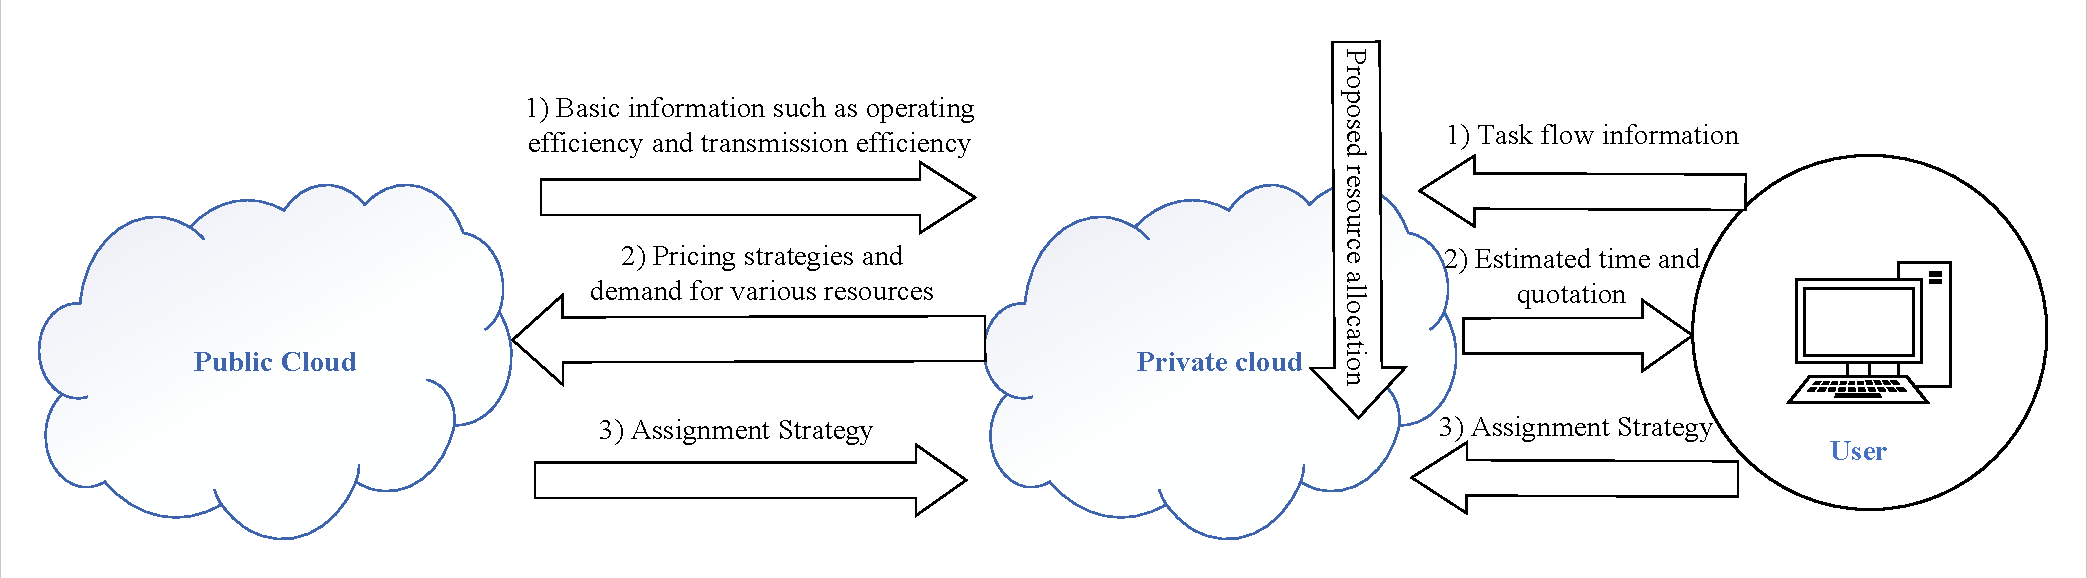
\includegraphics[width=\linewidth]{Stack.pdf}
    \caption{Illustration of the Stackelberg game model, depicting the hierarchical interaction between the public cloud (leader) and private clouds (followers)}
    \label{fig:placeholder}
\end{figure*}
\subsection{Data-Driven Adaptive Learning}
\label{sec:data_driven}

As serverless edge environments evolve into highly complex ecosystems characterized by time-varying wireless channel qualities, bursty task arrival patterns, and unpredictable user mobility, the assumption of stationarity required by traditional mathematical models often breaks down. Obtaining an accurate, closed-form expression for system transition probabilities becomes practically infeasible due to the sheer dimensionality of the state space. Consequently, data-driven approaches, particularly Deep Reinforcement Learning (DRL), have emerged as the dominant paradigm for addressing this "model-free" control problem. By formulating the function placement challenge as a Markov Decision Process (MDP), these methods enable the scheduler—acting as an intelligent agent—to learn optimal placement policies $\pi(a|s)$ directly through trial-and-error interactions with the environment. Unlike optimization-based methods that solve for a snapshot, DRL agents maximize long-term cumulative rewards, thereby implicitly learning to anticipate and adapt to system dynamics without requiring prior knowledge of the underlying physical laws.

\subsubsection{Model-Free Reinforcement Learning Strategies}
The landscape of model-free DRL is broadly divided into value-based and policy-based methods, each addressing specific aspects of the placement problem depending on the nature of the action space and the stability requirements.

Value-based methods, which aim to estimate the expected future reward (Q-value) of taking a specific action in a given state, serve as the foundational approach for discrete placement decisions. In the context of serverless computing, where the action space consists of selecting a discrete target node from a finite cluster, Deep Q-Networks (DQN) have proven highly effective. Traditional tabular Q-learning is severely limited by the curse of dimensionality when scaling to hundreds of edge nodes. To overcome this, Munir et al.~\cite{munir2019Edge} leveraged DQNs to approximate Q-values using deep neural networks, enabling scalable task assignment in complex scenarios where edge computing intersects with microgrid energy management. By using experience replay and target networks, such approaches stabilize the learning process against the inherent noise of edge telemetry.

However, a critical challenge in applying standard DQNs to online placement is the "greedy stagnation" phenomenon, where an agent over-exploits a known sub-optimal node while failing to discover potentially better resources due to a lack of exploration. Simple $\epsilon$-greedy strategies often fail to adapt quickly enough to rapid topology changes. To address this fundamental limitation, Zhang et al.~\cite{zhang2023Perturbed} proposed a specialized architecture: **DQN with Perturbed Rewards**. Integrating concepts from Multi-Armed Bandit (MAB) theory, this method injects stochastic noise into the reward signal during the training phase. This perturbation creates a "radius of exploration" around the estimated Q-values, forcing the agent to periodically test under-utilized nodes that might otherwise be ignored. This mechanism significantly enhances the robustness of the placement policy against dynamic server availability and prevents the system from converging to poor local optima. Furthermore, recent literature has increasingly adopted advanced variants such as Double DQN to mitigate overestimation bias and Dueling DQN to separate state-value estimation from action advantages, thereby refining the precision of offloading decisions in heterogeneous clusters.

In contrast, when the decision space becomes continuous or involves high-dimensional joint actions—such as the simultaneous optimization of discrete function placement and continuous transmission power control—value-based methods often struggle to find the global maximum. Policy-gradient methods offer a more viable solution in these high-complexity contexts by optimizing the policy function directly. For instance, Li et al.~\cite{li2020Proximal} leveraged the **Proximal Policy Optimization (PPO)** algorithm to tackle energy minimization in UAV-assisted edge computing. Unlike the aggressive updates of standard policy gradients, PPO employs a clipping mechanism to constrain the magnitude of policy updates within a "trust region." This ensures training stability even in highly volatile wireless environments where channel states fluctuate rapidly. Moreover, to accelerate convergence in large-scale distributed networks, architectures like Asynchronous Advantage Actor-Critic (A3C) have gained prominence. A3C allows multiple parallel agents to interact with different instances of the environment simultaneously, asynchronously updating a global policy. This parallelization effectively decorrelates the training data and allows the system to master complex placement tasks orders of magnitude faster than single-threaded learners.

\begin{figure*}[!t]
    \centering
    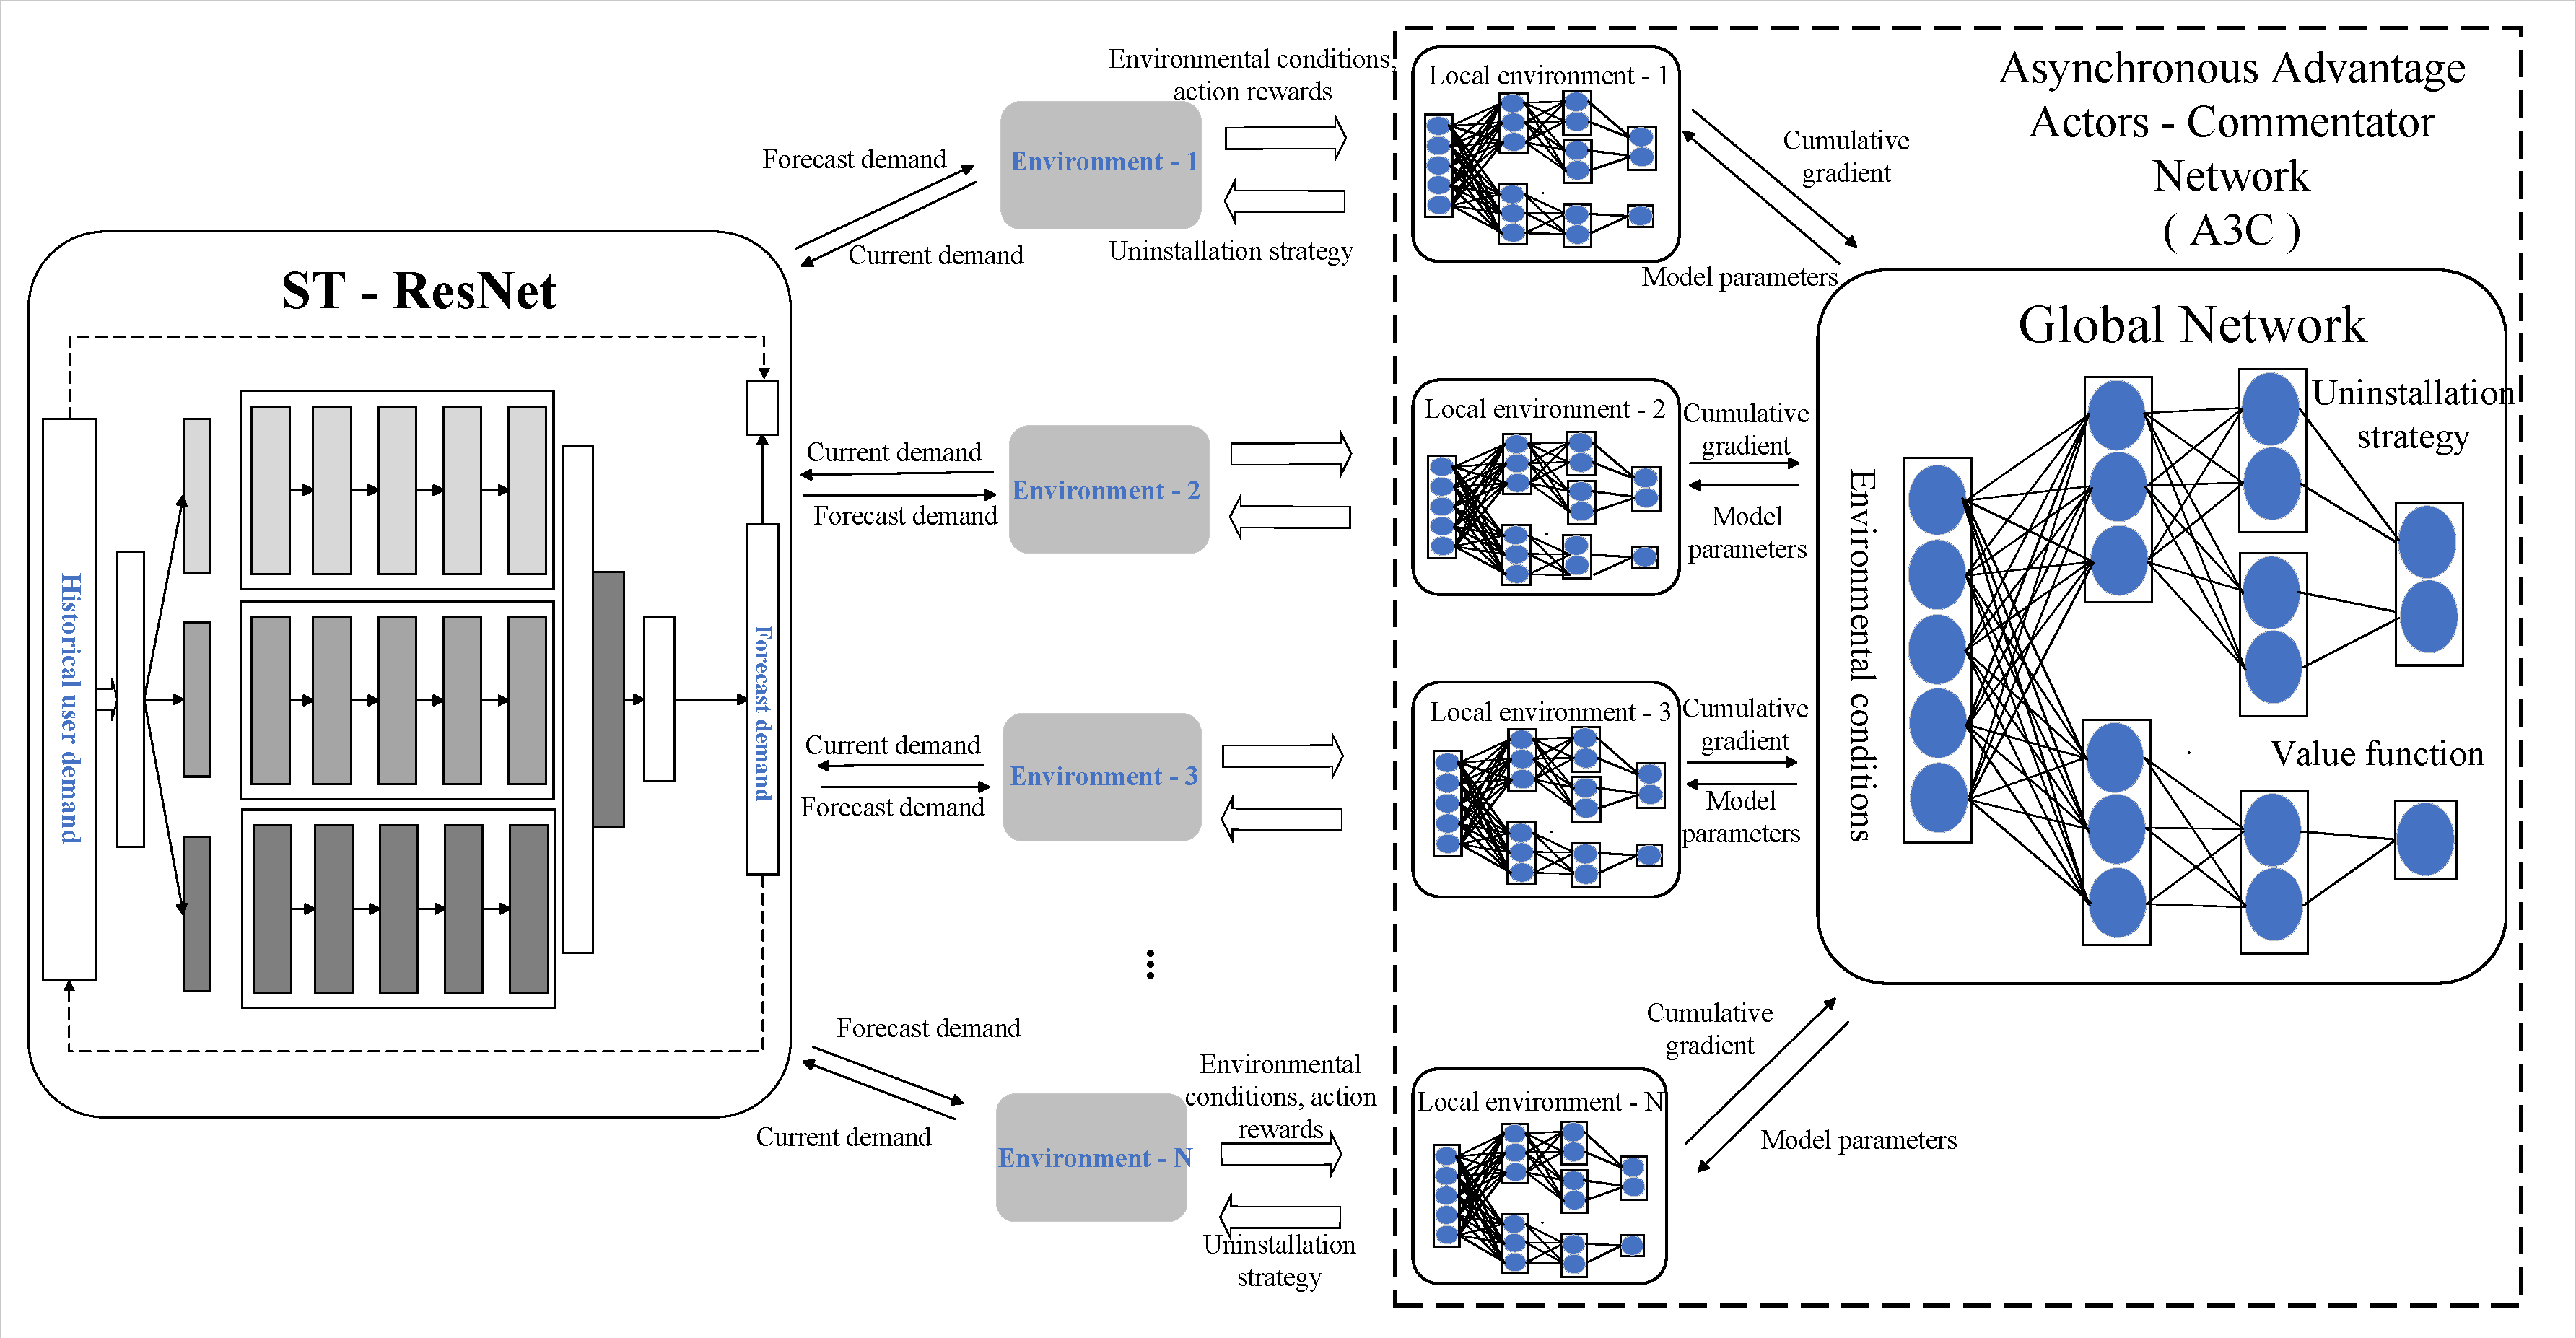
\includegraphics[width=1\linewidth]{CS.pdf}
    \caption{The framework of D-SOAC, illustrating how spatio-temporal prediction is integrated with the Actor-Critic network to enhance placement decisions.}
    \label{fig:dsoac_framework}
\end{figure*}

\subsubsection{State-Aware and Prediction-Enhanced Learning}
While standard DRL agents represent a significant leap forward, they typically operate in a reactive manner, making decisions based solely on the instantaneous snapshot of the system state. In serverless computing, where specific constraints like "Cold Start" latency and traffic burstiness act as critical bottlenecks, purely reactive policies often fail to meet stringent Service Level Agreements (SLAs). To bridge this gap, recent advancements have shifted towards "proactive" learning by augmenting the state space with predictive insights and structural awareness.

To mitigate the impact of bursty workloads, Xu et al.~\cite{xu2021DSOAC} pioneered the **D-SOAC (Distributed Service Offloading Actor-Critic)** framework. Recognizing that raw observation of current CPU load is insufficient for anticipating future congestion, they integrated a **Deep Spatio-Temporal Residual Network (ST-ResNet)** into the reinforcement learning loop. As illustrated in Fig.~\ref{fig:dsoac_framework}, this module does not merely act as a forecaster; it extracts complex temporal correlations (e.g., daily traffic periodicity) and spatial dependencies (e.g., user movement patterns between adjacent cells) from historical data. These high-level features are then fed as an augmented state vector into the Actor-Critic network. This fusion empowers the agent to pre-allocate resources before traffic spikes occur, effectively shifting the paradigm from reactive scheduling to predictive orchestration, which is crucial for maintaining low latency during peak hours.

Similarly, addressing the unique "scale-to-zero" characteristic of serverless platforms, Zhao et al.~\cite{zhao2024Cache} introduced **Structure-Aware DRL** via the C-DDQN (Cache-Based Double DQN) algorithm. Standard offloading algorithms often treat functions as generic computational loads, ignoring the substantial latency penalty incurred by initializing new function instances (cold start). C-DDQN fundamentally alters the MDP formulation by explicitly incorporating the "image caching status" of each edge node into the state representation. By perceiving which nodes already possess the necessary runtime environments or function images, the agent learns to prioritize "warm" nodes for placement. This structure-aware approach effectively transforms the placement problem into a joint optimization of computation offloading and cache management. Consequently, the agent can learn sophisticated behaviors, such as keeping frequently used containers alive or proactively migrating data to nodes with higher cache hit rates, significantly reducing the frequency of cold starts compared to generic, resource-blind DRL baselines.

\subsection{Rule-Driven Heuristics}
\label{sec:heuristics}

While model-driven approaches offer theoretical optimality guarantees and data-driven approaches provide adaptability to unknown dynamics, both paradigms frequently suffer from limitations that hinder their deployment in ultra-low latency scenarios: high computational complexity and extensive training overhead, respectively. For serverless edge computing, where decision-making must often occur within milliseconds to meet stringent Service Level Agreements (SLAs) and cope with the sheer volume of ephemeral function requests, rule-driven heuristics remain a cornerstone of industrial orchestration. These methods prioritize execution speed, implementation simplicity, and scalability, aiming to find feasible, near-optimal solutions for NP-hard placement problems in polynomial time. Unlike the "black-box" nature of neural networks, heuristics also offer high interpretability, allowing operators to understand exactly why a placement decision was made.

\subsubsection{Meta-Heuristic Search}
When the solution space is too vast for exact solvers but the quality of the solution cannot be entirely sacrificed for speed, meta-heuristics employ nature-inspired strategies to explore the landscape efficiently. These algorithms utilize stochastic processes to escape local optima, avoiding the combinatorial explosion typical of exact solvers like CPLEX or Gurobi.

One prominent class of meta-heuristics is **Swarm Intelligence**, which simulates the collective behavior of decentralized, self-organized systems. Zhu et al.~\cite{zhu2019Folo} addressed the service placement problem in vehicular fog computing using **Binary Particle Swarm Optimization (BPSO)**. Since the standard PSO algorithm operates in continuous space, it cannot be directly applied to the discrete nature of function placement (i.e., a function is either placed on a node or it is not). To overcome this, BPSO utilizes a sigmoid transfer function to map the continuous velocity of particles to probability values, which are then used to update the binary position vector of the solution. By iteratively adjusting placement schemes based on both personal best and global best experiences, the algorithm can jointly optimize conflicting objectives such as Quality of Service (QoS) and latency.

Parallel to swarm intelligence, **Evolutionary and Bio-inspired Algorithms** such as Genetic Algorithms (GA) and Ant Colony Optimization (ACO) have been widely cited in the literature (e.g., reviewed in \cite{hua2024Thesis}) for multi-objective placement. GA simulates the process of natural selection by encoding placement plans as chromosomes. Through operations like crossover (combining parts of two parent placement schemes) and mutation (randomly altering a node assignment), GA explores the solution space to evolve a population of high-quality solutions. This approach is particularly robust for generating Pareto-optimal fronts when trading off energy consumption against execution time. Similarly, ACO algorithms construct solutions by simulating ants traversing a graph, where edge nodes represent paths and pheromone levels represent the desirability of placing a function on a specific node. However, a key limitation shared by all meta-heuristics is their convergence speed; while significantly faster than exhaustive search, the iterative nature of these algorithms means they may still be too slow for the real-time processing of bursty, short-lived serverless requests compared to single-pass greedy rules.

\subsubsection{Constructive and Greedy Heuristics}
For scenarios requiring immediate decision-making, constructive heuristics build a solution step-by-step from scratch, typically making locally optimal choices at each stage without backtracking. These represent the fastest class of algorithms, typically operating with time complexities of $O(N)$ or $O(N \log N)$.

**Greedy Strategies** serve as the default logic for many container orchestrators (e.g., Kubernetes). Common strategies include \textit{Best-Fit}, which selects the node with the least remaining resources that still satisfies the function's requirements to minimize fragmentation, or \textit{Least-Loaded}, which balances traffic by selecting the node with the lowest CPU utilization. In the context of software-defined fog networks, Saha and Misra~\cite{saha2019SDF} formulated the placement problem as an Integer Linear Programming (ILP) model. Recognizing that solving the ILP is intractable for large-scale networks, they developed a specialized greedy heuristic. Their approach ranks candidate nodes based on a composite metric derived from resource availability and network proximity, iteratively assigning functions to the highest-ranked feasible node. While these greedy methods are extremely fast, they suffer from "myopia"—the tendency to make short-sighted decisions that optimize the current state but lead to load imbalances or resource bottlenecks in the long term.

A more specialized subclass of constructive heuristics in serverless computing is **Affinity-Based Rules**. These rules are specifically designed to address the "Cold Start" problem, a unique characteristic of FaaS platforms. When a function is triggered, if the target node does not have the relevant container image or a warm container, the system incurs a significant initialization latency. Affinity-based heuristics mitigate this by prioritizing \textit{Image Affinity} (placing functions on nodes that have already downloaded the function code) or \textit{Container Affinity} (placing functions on nodes with pre-warmed, idle containers). By effectively bypassing the expensive environment setup phase, these simple rule-based checks can yield latency improvements that rival complex optimization algorithms in cold-start-heavy workloads.

\subsubsection{Role as Baselines and Hybrids}
Although recent research interest has heavily pivoted toward Deep Reinforcement Learning (DRL), rule-driven heuristics continue to play two critical, evolving roles in the ecosystem of function placement algorithms.

First, they serve as essential **Baselines**. Heuristics provide a reliable "lower bound" for performance and an "upper bound" for execution speed in comparative experiments. Almost all learning-based studies (e.g., \cite{xu2021DSOAC}, \cite{li2020Proximal}) utilize GA or Greedy algorithms to benchmark the effectiveness of their proposed models. If a sophisticated DRL agent cannot outperform a simple greedy heuristic after convergence, it indicates a flaw in the reward design or state representation.

Second, and perhaps more importantly, heuristics are increasingly used in **Hybrid Initialization** and safety systems. Pure DRL agents often suffer from poor performance during the early stages of training (cold start problem in learning). To mitigate this, heuristics are used to generate high-quality initial experiences to pre-fill the replay buffer, allowing the DRL agent to start learning from a reasonable baseline rather than random noise. Furthermore, heuristics can act as a safety shield or "action mask" for AI models. In scenarios where the DRL agent has low confidence or suggests an unsafe action (e.g., overloading a critical node), the system can fall back to a reliable heuristic rule, thereby combining the optimality of AI with the stability and predictability of rule-based logic.

\begin{figure*}[!t]
    \centering
    \begin{tikzpicture}[
        % 定义样式
        >=Stealth, % 箭头样式
        node distance=1.5cm and 2cm,
        queue/.style={
            draw, rectangle, minimum width=2.5cm, minimum height=1cm,
            fill=white, thick
        },
        process/.style={
            draw, rectangle, rounded corners, minimum width=2.5cm, minimum height=1.2cm,
            align=center, fill=blue!10, thick
        },
        controller/.style={
            draw, ellipse, minimum width=3.5cm, minimum height=1.5cm,
            align=center, fill=green!10, thick, dashed
        },
        arrow/.style={->, thick, color=black!80},
        dashed_arrow/.style={->, thick, dashed, color=red!70}
    ]

    % 1. 绘制各个节点
    % 输入源
    \node (input) [align=center] {Stochastic\\Arrivals $A(t)$};

    % 队列 (画成一个带格子的缓冲区)
    \node (q_box) [queue, right=of input] {};
    % 在队列里画几条竖线代表积压的任务
    \foreach \x in {-0.8, -0.4, 0, 0.4}
        \draw[thick] ($(q_box.center)+(\x,-0.5)$) -- ($(q_box.center)+(\x,0.5)$);
    % 队列标签
    \node [above=0.1cm of q_box] {\textbf{Task Queue} $Q(t)$};
    \node [below=0.1cm of q_box, font=\footnotesize, color=gray] {Backlog Constraint};

    % 执行单元 (Service)
    \node (server) [process, right=of q_box] {\textbf{Execution Unit}\\Service Rate $\mu(t)$};

    % 输出 (分流)
    \node (local) [right=1.8cm of server, yshift=0.5cm] {Local CPU};
    \node (edge) [right=1.8cm of server, yshift=-0.5cm] {Edge/Cloud};

    % 控制器 (Lyapunov Controller)
    \node (ctrl) [controller, below=1.5cm of q_box] {
        \textbf{Lyapunov Controller}\\
        Min: $V \cdot \text{Cost}(t) + \Delta(\Theta(t))$
    };

    % 2. 绘制连接线
    % 到达 -> 队列
    \draw[arrow] (input) -- (q_box);
    
    % 队列 -> 执行
    \draw[arrow] (q_box) -- (server);

    % 执行 -> 输出 (分叉)
    \draw[arrow] (server.east) -- ++(0.5,0) |- (local.west);
    \draw[arrow] (server.east) -- ++(0.5,0) |- (edge.west);

    % 3. 绘制反馈回路 (核心逻辑)
    % 观测队列长度 (红虚线)
    \draw[dashed_arrow] (q_box.south) -- node[left, font=\footnotesize, color=black] {Observe $Q(t)$} (ctrl.north);
    
    % 控制决策 (蓝实线)
    \draw[arrow, color=blue!80] (ctrl.east) -| node[pos=0.3, above, font=\footnotesize, color=black] {Optimal Policy $\pi^*$} node[pos=0.3, below, font=\footnotesize, color=black] {(Offload / Power / Freq)} (server.south);

    % 4. 背景框 (可选，为了好看)
    \begin{pgfonlayer}{background}
        \node [draw=gray!30, fill=gray!5, fit=(q_box) (server) (ctrl), rounded corners, inner sep=0.5cm, dashed] (system) {};
        \node [above right, font=\itshape, color=gray] at (system.north west) {Edge Node System};
    \end{pgfonlayer}

    \end{tikzpicture}
    \caption{Conceptual framework of Lyapunov-based stochastic optimization for function placement. The controller dynamically adjusts the service strategy $\mu(t)$ by observing the current queue backlog $Q(t)$, balancing the trade-off between operational cost and system stability.}
    \label{fig:lyapunov_model}
\end{figure*}

\section{Comparative Analysis}
\label{sec:comparison}

The classification of function placement algorithms into model-driven, data-driven, and rule-driven paradigms reveals a fundamental diversity in how researchers tackle the challenges of serverless edge computing. No single approach serves as a "silver bullet"; rather, each paradigm occupies a distinct position in the multidimensional design space defined by solution quality, execution latency, environmental adaptability, and scalability. This section provides a critical synthesis of these trade-offs, analyzing how intrinsic algorithmic characteristics determine their applicability to specific serverless scenarios.

\subsection{Optimality versus Computational Latency}
The tension between the quality of the placement decision and the time required to compute it constitutes the primary trade-off in algorithm selection.

Model-driven approaches, particularly those based on convex optimization and Mixed-Integer Non-Linear Programming (MINLP), represent the theoretical gold standard for solution quality. As demonstrated in the works of Wang et al.~\cite{wang2021Lagrangian} and Tran and Pompili~\cite{tran2018MINLP}, these methods can converge to global or near-global optima, providing rigorous bounds on energy consumption and latency. However, this optimality comes at a steep computational cost. Since function placement is inherently NP-hard, the execution time of exact solvers grows exponentially with the cluster size. In the context of serverless computing, where functions are ephemeral and stateless, a solver taking seconds to optimize a function that runs for only milliseconds is practically infeasible. Consequently, exact optimization is best reserved for offline capacity planning or periodic long-term resource allocation rather than per-request scheduling.

In stark contrast, rule-driven heuristics prioritize speed above all else. Greedy strategies and constructive heuristics, such as those discussed in \cite{saha2019SDF}, operate with polynomial complexity, typically $O(N)$ or $O(N \log N)$. This allows them to make placement decisions in microseconds, satisfying the stringent real-time requirements of bursty serverless workloads. The inevitable downside is the "greedy gap"—the tendency to get trapped in local optima, potentially leading to resource fragmentation and load imbalance over time.

Data-driven learning, specifically Deep Reinforcement Learning (DRL), offers a compelling middle ground by shifting the computational burden from \textit{online inference} to \textit{offline training}. Although training a DRL agent requires significant computational resources and time, the trained policy network can infer near-optimal decisions rapidly via simple matrix operations. This "amortized" cost structure allows DRL to approximate the quality of optimization methods with the speed of heuristics, provided that the training environment accurately reflects real-world dynamics.

\subsection{Model Dependency and Environmental Robustness}
The efficacy of an algorithm is heavily contingent on the accuracy of the system information it possesses.

Model-driven optimization is fundamentally a "white-box" approach, relying on the assumption that system parameters—such as channel state information (CSI), interference patterns, and exact energy consumption models—are known and deterministic. In practical edge networks, obtaining such perfect information in real-time is often impossible due to measurement noise, privacy constraints, and signaling overhead. When the actual environment deviates even slightly from the mathematical model, the performance of optimization-based solutions can degrade precipitously.

Conversely, data-driven approaches operate as "black-box" solvers. Model-free RL algorithms, such as the PPO method used by Li et al.~\cite{li2020Proximal}, do not require explicit physical equations. Instead, they learn the underlying system dynamics implicitly through interaction and reward feedback. This gives them a significant advantage in heterogeneous environments where modeling complex interference or hardware idiosyncrasies is intractable. However, this robustness is purchased with "sample inefficiency." DRL agents often require millions of interaction steps to converge, leading to a "cold start" phase for the scheduler itself, where performance may be unstable until sufficient data is collected.
\begin{table*}[!t]
\centering
\caption{Qualitative Comparison of Function Placement Paradigms}
\label{tab:comparison}
\renewcommand{\arraystretch}{1.3}
\begin{tabular}{p{2.2cm} p{3.8cm} p{3.8cm} p{4.5cm}}
\toprule
\textbf{Paradigm} & \textbf{Key Strengths} & \textbf{Key Weaknesses} & \textbf{Ideal Use Cases} \\
\midrule
\textbf{Model-Driven} & 
Theoretical optimality guarantees; \newline Proven stability (Lyapunov); \newline Interpretability. & 
High computational complexity; \newline Reliance on accurate models; \newline Poor scalability to large clusters. & 
Offline capacity planning; Stability-critical control systems; Small-scale static clusters. \\
\hline
\textbf{Data-Driven} & 
High adaptability to dynamics; \newline Model-free robustness; \newline Fast online inference. & 
High training cost and data hunger; \newline Lack of explainability; \newline Unstable initial performance. & 
Highly dynamic, bursty workloads; Complex heterogeneous environments; Proactive resource scaling. \\
\hline
\textbf{Rule-Driven} & 
Ultra-low execution latency; \newline High scalability; \newline Ease of implementation. & 
Trapped in local optima; \newline Rigid, manual tuning required; \newline Myopic (short-sighted) decisions. & 
Real-time industrial orchestrators (e.g., K8s); Large-scale emergency scenarios; Baseline fallbacks. \\
\bottomrule
\end{tabular}
\end{table*}
\subsection{Adaptability to Dynamic Workloads}
Serverless edge environments are characterized by high dynamicity, including user mobility, time-varying channel qualities, and bursty request rates.

Traditional model-driven and heuristic approaches are typically \textit{reactive} and \textit{snapshot-based}. They optimize the placement for the current state of the network. If the network topology changes or a user moves to a new base station, the previous solution becomes invalid, necessitating a complete re-calculation. This "stop-and-compute" paradigm struggles to maintain continuity in highly mobile scenarios.

Data-driven methods, particularly those enhanced with prediction modules like D-SOAC~\cite{xu2021DSOAC}, introduce a \textit{proactive} paradigm. By integrating time-series forecasting (e.g., ST-ResNet or LSTMs) with decision-making, these algorithms can anticipate future traffic spikes or handover events. This capability is uniquely valuable for mitigating the "Cold Start" problem in serverless computing. While a heuristic might wait for a request to arrive before spinning up a container, a prediction-enhanced agent can pre-warm containers on the target edge node, thereby masking the initialization latency and ensuring seamless service continuity.

\subsection{Scalability and Cooperative Decision Making}
As the scale of the edge network expands, the dimensionality of the decision space becomes a critical bottleneck.

Centralized optimization and single-agent RL face the "curse of dimensionality," where the state-action space expands exponentially with the number of nodes. To address this, Multi-Agent Reinforcement Learning (MARL) and Game Theoretic approaches have gained prominence. Game theory, as applied in Stackelberg models \cite{sun2023Stackelberg}, provides a structured framework for decentralized decision-making, allowing users or edge nodes to optimize their local utility while converging to a Nash Equilibrium. Similarly, decomposition techniques in Lyapunov optimization allow large-scale global constraints to be broken down into distributed sub-problems. These decentralized paradigms are essential for future massive IoT networks, where a single central controller would become a performance bottleneck and a single point of failure.

\section{Open Challenges and Future Directions}
\label{sec:challenges}

While significant strides have been made in modeling, learning, and optimizing function placement for serverless edge computing, the transition from theoretical frameworks to production-grade deployment faces several formidable hurdles. The current body of literature often isolates specific sub-problems, neglecting the intricate coupling between placement decisions and broader system dynamics. This section identifies critical gaps in existing research and outlines promising avenues for future exploration, emphasizing the need for holistic orchestration, dependency awareness, and decentralized intelligence.

\subsection{Joint Optimization of Placement and Cold Start Mitigation}
A prevailing limitation in many existing model-driven and rule-driven approaches is the decoupling of function placement from container lifecycle management. Traditional algorithms often assume that computing resources are "ready-to-use" or treat the initialization latency as a static penalty. However, in serverless environments, the "Cold Start" latency—incurred by downloading code packages and starting containers—can be orders of magnitude higher than the actual execution time. 

Future research must move towards the \textit{joint optimization} of function placement and proactive caching strategies. Rather than treating placement and auto-scaling as separate control loops, next-generation algorithms should aim to output a composite decision vector: determining not only \textit{where} to place a function but also \textit{when} to pre-warm a container or \textit{where} to cache a function image. Although prediction-enhanced methods like D-SOAC have begun to address proactive scaling, there is a need for more granular "keep-alive" strategies that balance memory consumption with latency reduction across the edge-cloud continuum.

\subsection{Dependency-Aware Scheduling for Complex Workflows}
Current research frequently simplifies the workload model by treating serverless functions as independent, atomic tasks. In reality, modern cloud-native applications are structured as complex workflows or Directed Acyclic Graphs (DAGs), where the output of one function triggers the execution of another. When interdependent functions are dispersed across geographically distributed edge nodes without considering their communication overhead, the resulting network latency can negate the benefits of computation offloading.

Addressing this challenge requires a paradigm shift from task-centric to \textit{workflow-centric} placement. Future algorithms need to incorporate graph partitioning and topology awareness into their decision logic. For instance, data-driven agents could be designed to recognize frequent invocation patterns, automatically learning to "co-locate" highly coupled functions on the same node or within the same local area network. Furthermore, exploring the trade-offs between "function fusion" (merging multiple functions into one container) and distributed execution offers a fertile ground for optimizing DAG-based serverless applications.

\subsection{Scalability via Decentralized Multi-Agent Collaboration}
As the scale of the Internet of Things (IoT) expands, the centralized decision-making architectures employed by many current DRL and optimization approaches face a critical scalability bottleneck. A single central controller collecting state information from thousands of edge nodes inevitably suffers from communication congestion, processing delays, and single-point-of-failure risks.

The future of massive-scale serverless orchestration lies in \textit{decentralized and collaborative intelligence}. There is a pressing need to advance Multi-Agent Reinforcement Learning (MARL) frameworks where edge nodes act as autonomous agents. Research should focus on overcoming the non-stationarity problem in MARL, where the environment changes due to the simultaneous actions of other agents. Techniques such as mean-field game theory and federated learning could be instrumental here. Specifically, Federated Learning (FL) offers a promising direction by allowing agents to collaboratively train a shared placement policy without exchanging raw telemetry data, thereby enhancing both scalability and bandwidth efficiency.

\subsection{Privacy-Preserving and Security-Aware Placement}
The majority of existing studies optimize primarily for performance metrics such as latency, energy, or cost, often overlooking security and privacy constraints. However, edge computing inherently involves processing sensitive data (e.g., healthcare monitoring, smart home video) on dispersed infrastructure. Placing a function processing private data onto an untrusted or insecure edge node poses severe compliance risks.

Future placement algorithms must incorporate security as a hard constraint rather than an afterthought. This involves developing "trust-aware" placement mechanisms that consider data sovereignty laws (e.g., GDPR) and the security certification levels of edge nodes. Optimization models should be extended to include privacy budgets or trust scores as constraints. Additionally, in learning-based approaches, ensuring that the training process itself does not leak sensitive workload patterns to potential adversaries remains an open challenge. The integration of Trusted Execution Environments (TEEs) with function scheduling logic represents a critical step towards secure serverless edge computing.


\section{Conclusion}
\label{sec:conclusion}

The paradigm shift towards serverless edge computing has fundamentally reshaped the landscape of distributed application deployment, promising a future of ultra-low latency and seamless scalability. However, realizing this vision requires overcoming substantial orchestration hurdles, primarily the complex mapping of fine-grained, stateless functions onto heterogeneous and resource-constrained edge nodes. This survey has systematically explored the state-of-the-art in function placement algorithms, bridging the critical gap between theoretical mathematical formulations and the practical exigencies of dynamic production environments.

Through the proposal of a novel \textbf{Hybrid Taxonomy}, we have synthesized existing research into three distinct paradigms, each offering unique strengths in the multidimensional trade-off space of optimality, adaptability, and execution speed. Our analysis reveals that \textbf{Model-Driven Theoretical Optimization}, utilizing frameworks such as convex optimization and Lyapunov control, remains the gold standard for scenarios requiring rigorous stability guarantees and multi-user fairness. Yet, its practical utility is often constrained by the necessity for accurate system modeling and the high computational cost of solving NP-hard problems in real-time. Conversely, the rapid ascent of \textbf{Data-Driven Adaptive Learning}, particularly Deep Reinforcement Learning (DRL), has provided a robust solution for managing environmental uncertainty and "black-box" dynamics. By integrating prediction modules and structure-aware state representations, these methods have shifted the paradigm from reactive to proactive scheduling, albeit at the cost of high training overhead and sample inefficiency. Meanwhile, \textbf{Rule-Driven Heuristics} continue to serve as an indispensable backbone for industrial orchestrators, offering the requisite scalability and sub-millisecond decision latency that rigorous optimization and heavy learning models struggle to achieve.

Critically, this survey highlights that the future of serverless function placement does not lie in the dominance of a single algorithmic approach, but rather in the **convergence and hybridization** of these paradigms. The current "siloed" approach—where placement, cold-start mitigation, and security are treated as separate optimization objectives—is becoming increasingly insufficient. The next generation of placement algorithms must evolve towards holistic orchestration. This entails the joint optimization of function placement with container lifecycle management to neutralize cold start latencies, the adoption of workflow-centric scheduling to minimize communication overhead in complex DAGs, and the integration of privacy constraints into the decision logic. Furthermore, as edge networks scale to massive IoT deployments, the transition from centralized controllers to decentralized, multi-agent collaborative intelligence will be paramount. By addressing these open challenges, future research will pave the way for a truly autonomous, resilient, and ubiquitous serverless edge ecosystem.

% --- Bibliography ---
\begin{thebibliography}{10}
\bibliographystyle{IEEEtran}

% [3.1.1] Static Snapshot & Convex Optimization
\bibitem{wang2021Lagrangian}
Y.~Wang, K.~Wang, H.~Huang, T.~Miyazaki, and S.~Guo, ``Traffic and computation co-offloading with energy harvesting in software-defined cellular networks,'' \emph{IEEE Trans. Wireless Commun.}, vol.~20, no.~7, pp. 4467--4480, 2021.

\bibitem{zhang2020Difference}
H.~Zhang, Z.~Zhang, H.~Dai, K.~Long, and G.~K.~Karagiannidis, ``Power allocation and cache placement for NOMA-based mobile edge computing,'' \emph{IEEE Commun. Lett.}, vol.~24, no.~10, pp. 2260--2264, 2020.

\bibitem{tran2018MINLP}
T.~X.~Tran and D.~Pompili, ``Joint task offloading and resource allocation for multi-server mobile-edge computing networks,'' \emph{IEEE Trans. Veh. Technol.}, vol.~68, no.~1, pp. 856--868, 2018.

\bibitem{du2018Computation}
J.~Du, L.~Zhao, J.~Feng, and X.~Chu, ``Computation offloading and resource allocation in mixed fog/cloud computing systems with min-max fairness guarantee,'' \emph{IEEE Trans. Commun.}, vol.~66, no.~4, pp. 1594--1608, 2018.

\bibitem{deng2015Towards}
R.~Deng, R.~Lu, C.~Lai, T.~H.~Luan, and H.~Liang, ``Optimal workload allocation in fog-cloud computing toward balanced delay and power consumption,'' \emph{IEEE Internet Things J.}, vol.~3, no.~6, pp. 1171--1181, 2016.

% [3.1.2] Lyapunov Optimization
\bibitem{chen2022Lyapunov}
H.~Chen, Y.~Zhang, Z.~Wang, and D.~Wu, ``Energy-efficient service selection and energy storage management for mobile edge computing,'' \emph{IEEE Trans. Green Commun. Netw.}, vol.~6, no.~1, pp. 312--325, 2022.

\bibitem{tang2023Wireless}
D.~Tang, H.~Huang, Z.~Luo, et al., ``Wireless power transfer assisted computation offloading in mobile edge computing,'' \emph{IEEE Trans. Commun.}, vol.~71, no.~4, pp. 2105--2118, 2023.

\bibitem{wang2022Edge}
Y.~Wang, S.~Guo, Z.~Zheng, et al., ``Edge-cloud resource coordination for energy-efficient computation offloading,'' \emph{IEEE Trans. Serv. Comput.}, vol.~15, no.~2, pp. 1089--1102, 2022.

\bibitem{zhao2018FEMOS}
S.~Zhao, Y.~Yang, Z.~Shao, X.~Yang, H.~Qian, and C.~Xu, ``FEMOS: Fog-enabled multitier operations scheduling in dynamic wireless networks,'' \emph{IEEE Internet Things J.}, vol.~5, no.~2, pp. 1169--1183, 2018.

% [3.1.3] Game Theory
\bibitem{sun2023Stackelberg}
W.~Sun, Z.~Zhang, and H.~Jiang, ``A double-layer Stackelberg game for computation offloading in vehicular edge computing,'' \emph{IEEE Trans. Veh. Technol.}, vol.~72, no.~3, pp. 3892--3905, 2023.

\bibitem{zhang2018Joint}
K.~Zhang, Y.~Mao, S.~Leng, Y.~He, and Y.~Zhang, ``Optimal delay constrained offloading for vehicular edge computing networks,'' in \emph{Proc. IEEE ICC}, 2017, pp. 1--6.

\bibitem{cao2022V2X}
B.~Cao, J.~Zhao, Y.~Gu, et al., ``Distributed multiuser computation offloading for cloudlet-based mobile cloud computing: A game-theoretic approach,'' \emph{IEEE Trans. Veh. Technol.}, vol.~67, no.~1, pp. 752--764, 2018.

\bibitem{zhang2023Exact}
X.~Zhang, W.~Zhang, and Z.~Chen, ``Exact potential game for multi-user computation offloading in edge computing,'' \emph{IEEE Trans. Mobile Comput.}, vol.~22, no.~5, pp. 2890--2903, 2023.

\bibitem{chen2023Potential}
Y.~Chen, D.~Wu, and Y.~Zhang, ``TUSGT: A two-way update strategy based on game theory for task offloading in edge computing,'' \emph{Comput. Sci.}, vol.~50, no.~2, pp. 32--41, 2023.

% [3.2.1] DRL (Value & Policy)
\bibitem{sen2019Machine}
T.~Sen and H.~Shen, ``Machine learning based timeliness-guaranteed and energy-efficient task assignment in edge computing systems,'' in \emph{Proc. IEEE ICFEC}, 2019, pp. 1--10.

\bibitem{dab2019QLearning}
B.~Dab, N.~Aitsaadi, and R.~Langar, ``Q-learning algorithm for joint computation offloading and resource allocation in edge cloud,'' in \emph{Proc. IFIP/IEEE IM}, 2019, pp. 45--52.

\bibitem{munir2019Edge}
M.~S.~Munir, S.~F.~Abedin, N.~H.~Tran, et al., ``When edge computing meets microgrid: A deep reinforcement learning approach,'' \emph{IEEE Internet Things J.}, vol.~6, no.~5, pp. 7360--7374, 2019.

\bibitem{zhang2023Perturbed}
F.~Zhang, G.~Liu, and X.~Fu, ``Delay-aware task scheduling in edge computing based on deep reinforcement learning with perturbed rewards,'' \emph{IEEE Trans. Netw. Service Manag.}, vol.~20, no.~1, pp. 560--572, 2023.

\bibitem{li2020Proximal}
M.~Li, J.~Cheng, J.~Wang, et al., ``Energy-efficient UAV-assisted mobile edge computing via proximal policy optimization,'' \emph{IEEE Trans. Wireless Commun.}, vol.~19, no.~9, pp. 6158--6172, 2020.

% [3.2.2] Prediction & Structure Aware
\bibitem{xu2021DSOAC}
X.~Xu, Z.~Fang, L.~Qi, et al., ``A distributed service offloading method using deep reinforcement learning for edge computing,'' \emph{Chin. J. Comput.}, vol.~44, no.~12, pp. 2382--2405, 2021.

\bibitem{zhao2024Cache}
T.~Zhao, B.~Zhou, and W.~Li, ``Cache-based double deep Q-network for service placement in mobile edge computing,'' \emph{Comput. Sci.}, vol.~51, no.~2, pp. 300--310, 2024.

% [3.3] Heuristics & Thesis
\bibitem{zhu2019Folo}
C.~Zhu, G.~Pastor, Y.~Xiao, et al., ``Folo: Latency and quality optimized task allocation in vehicular fog computing,'' \emph{IEEE Internet Things J.}, vol.~6, no.~3, pp. 4150--4161, 2019.

\bibitem{hua2024Thesis}
X.~Hua, ``Serverless function placement optimization based on deep reinforcement learning,'' Master's thesis, School of Comput. Sci. Tech., China Univ. Mining Technol., Xuzhou, China, 2024.

\bibitem{saha2019SDF}
S.~Saha and S.~Misra, ``Detour: Dynamic task offloading in software-defined fog for IoT applications,'' \emph{IEEE J. Sel. Areas Commun.}, vol.~37, no.~5, pp. 1159--1166, 2019.

\end{thebibliography}
\end{document}



